\chapter{Aggregated Signature Based Set Membership Proofs}
\label{ch:AggSM}
\label{sec:ConstructAggregation}
%TODO fix intro
In the previous chapter  general description and definition of aggregated set membership proofs was described. In this chapter this general formulation will be used to propose a construction to aggregated a specific construction of set membership proof. More precisely it is investigated if the non-interactive construction of the set membership proposed in \cite{Efficient_proof_interval} can be aggregated according to Definition \ref{def:GeneralAggregation} such that it satisfies the completeness, soundness and zero knowledge in Definition \ref{def:ZKP_agg}. The specific set membership that will be considered is the signature based set membership in Construction \ref{alg:ZKSM}.

%It is seen that the verification algorithm in Construction \ref{alg:VAHSS-HSS-RP} will be time consuming, since each client is verified individually. Therefore a desired property for the above presented server and clients verifiable AHSS would be to aggregate the range proofs into one, since then the verifier would have to perform one range proof verification instead of one for each client as in Construction \ref{alg:VAHSS-HSS-RP}. This would decrease the runtime for the verification significantly, especially in implementations where many clients participate. 
%TODO require the aggregated to filfil def 4. 
%Aggregating the range proofs would require the proofs to be homomorphic, such that the verification remains valid also for an aggregated proof.

\section{Aggregation of signature based set membership proof}


The considred set membership proofs can be used to construct a signature-based range proof as discussed previously and proposed in \cite{Efficient_proof_interval}. The strong similarity between the set membership proof and the derived range proof results in that the results obtained for the public signature based set membership proofs can easily be adjusted to also hold for the  for the signature-based range proof. This would then result in an aggregated range proof construction. Such a construction is not further investigates in this paper but it is stressed that the results follow directly from the results for the public signature based set membership proofs. 

%In this section the possibility to aggregate the set membership and signature based range proofs  is examined.  The construction of these two are similar and it is sufficient to consider one of them and the conclusion will hold for both constructions. Due to its simpler notation the set membership proof is considered.

To aggregate the public signature based set membership proofs possible constructions for the algorithm \textbf{Aggregate} is evaluated. The starting point for designing such a construction is that the aggregation of public signature set membership proofs according to the algorithm \textbf{Aggregate} should result in construction that satisfies the completeness requirement in Definition \ref{def:ZKP_agg}. Remark that it is assumed that the verification of the aggregated proof should be designed in the same way as the algorithm \textbf{Verify} in Construction \ref{alg:ZKSM}. Having found an implementation of the algorithm \textbf{Aggregate} that satisfies the completeness it will then be examined under what assumptions the soundness and zero knowledge in Definition \ref{def:ZKP_agg} is satisfied. 

To investigate different designs of the algorithm \textbf{Aggregate} and whether it  provides an aggregated set membership proof that satisfies the completeness the following is considered. 

Two set membership proof $\Sigma_1$ and $\Sigma_2$ generated by the algorithm \textbf{Prove} in construction \ref{alg:ZKSM}, recall that the proofs are on the form $\Sigma_i = (V_i,a_i,D_i,z_{x_i},z_{\tau _i},z_{R_i}, )$ for $i=1,2$. In addition to the proofs also assume that $C_i$ for $i=1,2$ are two Pedersen commitments  published by the provers, $p_1$ and $p_2$, hiding the secrets $x_1$,$x_2$. The public parameters, $pp$, are generated by the algorithm \textbf{SetUp} in Construction \ref{alg:ZKSM}  and that the challenges $c_i, \:i=1,2$ which can be computed as a hash of the proofs. 

Since it will be assumed that the verification of an aggregated public signature based set membership proofs is performed as the algorithm \textbf{Verify} in Construction \ref{alg:ZKSM} the completeness property holds if an aggregates proof $\Sigma_a = (C,a,D,z_x,z_\tau,z_R)$ satisfies the two equalities  $D=C^{c}h^{z_{R}}g^{z_{x}}\wedge a = e(V,y)^ce(V,g)^{z_{x}}e(g,g)^{z_{\tau}}$, where $C=C_1C_2$ and $c=c_1c_2$.  Note that to reduce notation subscripts on the proof elements is omitted,

%TODO verify starting with correctness
%To aggregate the proof all elements constructing the proof would need to be aggregated such that the verification of the aggregated proof can be carried out in the same without aggregation. 

%TODO snygga till formulering nedan
The simplest design of the algorithm \textbf{Aggregate} for the two considered set membership proofs would be define the aggregated set membership proof as the element-wise product of the two set membership proofs. This yields an aggregated set membership proof on the form, $\Sigma_a = (V,a,D,z_{x},z_{\tau },z_{R})$,  where $V, a, D,z_{x},z_{\tau },z_{R}$ are computed as,
\begin{equation}
\begin{aligned}
\label{eq:naiveAgg}
V =& V_1V_2 = g^{\frac{\tau_1}{\chi + x_1}}g^{\frac{\tau_2}{\chi + x_2}}  = g^{\frac{\tau_1}{\chi + x_1} + \frac{\tau_2}{\chi + x_2}}  \\
a =& a_1a_2 = \big(e(V_1,g)^{-s_1})e(g,g)^{t_1}\big)  \big(e(V_2,g)^{-s_2})e(g,g)^{t_2}\big) \\
=&  \big( e(g,g)^{\frac{-s_1\tau_i}{\chi+x_1}}e(g,g)^{t_1}\big) \big( e(g,g)^{\frac{-s_2\tau_2}{\chi+x_2}}e(g,g)^{t_2}\big) \\
D =& D_1D_2 = ( g^{s_1}h^{m_1} ) (g^{s_2} h^{m_2}) = g^{s_1+s_2}h^{m_1+m_2}\\
z_x =& z_{x_1} + z_{x_2} = (s_1-c_1x_1)+(s_2-c_2x_2)\\
z_R =& z_{R_1} + z_{R_2} = (m_1-c_1R_1)+(m_2-c_2R_2)\\
z_\tau =& z_{x_1} + z_{x_2} = (t_1-c_1\tau_1)+(t_2-c_2\tau_2)\\ 
\end{aligned} 
\end{equation}
%are the multiplication of the corresponding elements in the two non aggregated range proofs and are the addition of the corresponding elements in the two non aggregated range proofs. To clarify two examples are, $D=D_1*D_2 =g^{s_1}h^{m_1}*g^{s_2}h^{m_2} = g^{s_1+s_2}h^{m_1+m_2}$, and the two exponentials are now refereed to as $s,m$, more over $z_x = z_{x_1}+z_{x_2} = (s_1-x_1c_1 )+ (s_2-x_2c_2) = s- x_1c_1-x_2c_2 $.
Further assume that the  challenges $c_1$ and $c_2$ has been calculated according to $c_i=Hash(C_i,V_i,a_i,D_i),\: i=1,2$.
% and remember that the  commitments $C_i$  are homomorphic, which follows directly from the homomorphic properties of the Pedersen commitment. It is less obvious to see that the bilinear map can be aggregated, but this has been shown and the security proven in \cite{aggregate_bm}. However the homomorphic properties of the Pedersen commitment and bilinear maps does not guarantee that the set membership proofs are homomorphic. 


%But although bilinear maps can be aggregated it turns out that the set membership proof does not have this property, this follows from design of $z_x,z_\tau $ and $z_R$ using addition and subtraction, when multiplying two sums the cross-terms will not cancel as desired, this is seen below. 

Next it will be investigated if the aggregated proof $\Sigma_a$ derived as above satisfies the completeness in Definition \ref{def:ZKP_agg}. For the considered set membership proof this means that it must hold that, $1)$ $D \overset{?}{=} C^ch^{z_R}g^{z_x}$ and $2)$ $ a \overset{?}{=} e(V,y)^ce(V,g)^{-z_x}e(g,g)^{z_\tau}$. Evaluating the first of the two equalities it follows that,
\begin{align*}
LHS &= D = D_1*D_2 = g^{s_1+s_2}*h^{m_1+m_2} \\
RHS &= C^ch^{z_R}g^{z_x} = (C_1*C_2)^{c_1c_2}h^{z_{R_1}+z_{R_2}}g^{z_{x_1}+z_{x_2}} \\ 
&=(g^{x_1}h^{R_1}g^{x_2}h^{R_2}) ^{c_1c_2}  h^{m_1-R_1c_1+m_2-R_2c_2} g^{s_1- x_1c_1+s_2-x_2c_2} \\
&= g^{c_1c_1(x_1+x_2)+s_1+s_2-x_1c_1-x_2c_2}h^{c_1c_2(R_1+R_2)+m-R_1c_1-R_2c_2} \\
\implies \text{LHS}\neq \text{RHS}.
\end{align*}

The completeness property is not satisfied given an aggregation on the form in equation \eqref{eq:naiveAgg}. Studying the LHS and RHS above it is noted that the equality does not hold since  $ c_1c_2(x_1+x_2) = c_1c_2x_1+c_1c_2x_2 \neq x_1c_1 + x_2c_2$. Further note that if $c_1=c_2$ then this would be easy to fix. Clearly it cannot be guaranteed that the challenges for two different set membership proofs will be equal since they depend on randomness in the proof construction. However having pinpointing this source of inequality an aggregation that circumvent this issue is seeked.

Again consider the two set membership proofs $\Sigma_1,\Sigma_2$ as defined above, but now restrict the aggregation to only concern half the set membership proof. Namely only terms participating in the the first equality check, $D\overset{?}{=} C^ch^{z_R}g^{z_x}$, in the verification. 

Note that if only a part of the proofs are aggregated it still leads to reduction of computational complexity for the verifier. The goal is now design the aggregation such that the aggregated proof satisfies $D = C^ch^{z_R}g^{z_x}$. 
%Before aggregation calculate the challenges $c_1,c_1$ as $c_i =Hash(D_i,a_i),\:i=1,2$. 
Define the aggregated proof as, $\Sigma_a=(D,z_x,z_R)$, this means the proof does not contain the bilinear maps output $a$ and the group element $V, z_{\tau}$. Further let the the aggregated proof be computed according to, 
\begin{equation}
\label{eq:aggD2}
\begin{aligned}
D &= D_1^{c_2}\cdot D_2^{c_1} = (g^{s_1}h^{m_1}) ^{c_2} \cdot (g^{s_2}h^{m_2}) ^{c_1}  =g^{s_1c_2+s_2c_1}h^{m_1c_2+m_2c_1} \\
z_x &= c_2z_{x_1} +c_1 z_{x_2} = c_2(s_1-x_1c_1)  + c_1(s_2-x_2c_2) = s_1c_2 + s_2c_1 -c_1c_2(x_1+x_2)\\
z_R &= c_2z_{R_1} +c_1 z_{R_2} = c_2(m_1-R_1c_1)  + c_1(m_2-R_2c_2) = m_1c_2 + m_2c_1 -c_1c_2(R_1+R_2)
\end{aligned}
\end{equation}
This construction of the aggregation will result in that the challenges always appears in a product which resolves the problem of them being different. Additionally also define the product of the challenges and commitments as,
\begin{align*}
c &= c_1c_2 \\
C &= C_1C_2 = (g^{x_1}h^{R_1}) (g^{x_2}h^{R_2}) = g^{x_1+x_2}h^{R_1+R_2}.
\end{align*}

%It is assumed that the random values $R_i$ is chosen such that $R_n = \phi(N)\lceil \frac{\sum_{i=1}^{n-1}R_i}{\phi(N)}\rceil- \sum_{i=1}^{n-1}R_i $, which holds for the randomness in a VHASS construction, hence for $i=1,2$ if follows that $R_2 = \phi(N)\lceil \frac{R_1}{\phi(N)}\rceil- R_1$, and thus $h^{c_1c_2(R_1+R_2)} = 1$. 
%This property will not be required for the below calculations, however is does reduce notation and therefore the computations are done under this assumption. 

The aggregated proof $\Sigma_a$, computed according to equation \eqref{eq:aggD2} satisfies the equality $D= C^ch^{z_R}g^{z_x}$, this is seen below,
\begin{align*}
LHS &= D = D_1^{c_2}\cdot D_2^{c_1} =g^{s_1c_2+s_2c_1}h^{m_1c_2+m_2c_1} \\
RHS &= C^ch^{z_R}g^{z_x} = (C_1C_2)^{c_1c_2}h^{c_2z_{R_1}+c_1z_{R_2}}g^{c_2z_{x_1}+c_1z_{x_2}}\\ 
&=(g^{x_1 + x_2})^{c_1c_2} h^{m_1c_2 +m_2c_1} g^{s_1c_2+ s_2c_1- c_1c_2(x_1+x_2)}  \\
&= g^{(x_1+x_2)c_1c_2 - c_1c_2(x_1+x_2) +s_1c_2+s_2c_1} h^{m_1c_2 +m_2c_1} = g^{s_1c_2+s_2c_1} h^{m_1c_2 +m_2c_1} \\
\\ \implies \text{LHS} =\text{RHS}&.
\end{align*}

%This means that this aggregation to construct the proof $RP$ , from the two range proofs $RP_1,RP_2$ as above satisfies the first equality of the verification. 
Aggregation of the two set membership proof defined according to equation  \eqref{eq:aggD2} results in an aggregation that satisfies the  completeness. The next step is to check if this aggregation can be extended to aggregate an arbitrary number of set membership proofs and still satisfy the completeness. 

Consider $|\mathcal{S}|$ provers and consequently  $|\mathcal{S}|$ set membership proofs denoted $\Sigma_i,\: i\in\mathcal{S}$. The aggregation in equation \eqref{eq:aggD2} extended to aggregate all proof results in the aggregation procedure below,
\begin{equation}
\label{eq:aggDn}
\begin{aligned}
D &=\prod_{i\in\mathcal{S}}  D_i ^{\prod_{\substack{j\in\mathcal{S}\\ j\neq i}} c_j }  =  \prod_{i\in\mathcal{S}}  (g^{s_i}h^{m_i}) ^{\prod_{\substack{j\in\mathcal{S}\\ j\neq i}}  c_j } = g ^ {\sum_{i\in\mathcal{S}} \Big(\prod_{\substack{j\in\mathcal{S}\\ j\neq i}}   c_j \Big)s_i} h^ {\sum_{i\in\mathcal{S}} \Big(\prod_{\substack{j\in\mathcal{S}\\ j\neq i}}   c_j \Big)m_i} \\
z_x &= \sum_{i\in\mathcal{S}} \Big( \prod_{\substack{j\in\mathcal{S}\\ j\neq i}} c_j \Big) z_{x_i} = \sum_{i\in\mathcal{S}} \Big( \prod_{\substack{j\in\mathcal{S}\\ j\neq i}} c_j \Big)s_i - \big( \prod_{j\in\mathcal{S}} c_j \big) \sum_{i\in\mathcal{S}} x_i\\
z_R &=  \sum_{i\in\mathcal{S}}  \Big( \prod_{\substack{j\in\mathcal{S}\\ j\neq i}} c_j \Big) z_{R_i} = \sum_{i\in\mathcal{S}} \Big( \prod_{\substack{j\in\mathcal{S}\\ j\neq i}} c_j \Big)m_i - \big( \prod_{j\in\mathcal{S}} c_j \big) \sum_{i\in\mathcal{S}} R_i 
\end{aligned}
\end{equation}
Let $C=\prod_{i\in\mathcal{S}} C_i$ be the product of all Pedersen commitments and $c= \prod_{i\in\mathcal{S}} c_i$ the product of the challenges.  The partly aggregated set membership proof $\Sigma_a = (D,z_x,z_r)$ computed according to equation \ref{eq:aggDn} satisfies $D= C^ch^{z_R}g^{z_x}$, 
\begin{align*}
LHS =& D = g ^ {\sum_{i\in\mathcal{S}} \Big(\prod_{\substack{j\in\mathcal{S}\\ j\neq i}}   c_j \Big)s_i} h^ {\sum_{i\in\mathcal{S}} \Big(\prod_{\substack{j\in\mathcal{S}\\ j\neq i}}    c_j \Big)m_i}  
\\
RHS =& C^ch^{z_R}g^{z_x} =  \Big( \prod_{i\in\mathcal{S}} C_i \Big)^{\prod_{i\in\mathcal{S}} c_i}h^ {\sum_{i\in\mathcal{S}} \Big( \prod_{\substack{j\in\mathcal{S}\\ j\neq i}}   c_j \Big)m_i}
\\
&g^{ \sum_{i\in\mathcal{S}} \Big( \prod_{\substack{j\in\mathcal{S}\\ j\neq i}}   c_j \Big)s_i - \big( \prod_{j\in\mathcal{S}} c_j \big) \sum_{i\in\mathcal{S}} x_i}
\\ 
 =& \Big( g^{\sum_{i\in\mathcal{S}} x_i} h^{\sum_{i\in\mathcal{S}} R_i}\Big)^{\prod_{i\in\mathcal{S}} c_i} h^{ \sum_{i\in\mathcal{S}} \Big( \prod_{\substack{j\in\mathcal{S}\\ j\neq i}} c_j \Big)m_i - \big( \prod_{j\in\mathcal{S}} c_j \Big) \sum_{i\in\mathcal{S}} R_i  }
 \\
 &g^{ \sum_{i\in\mathcal{S}} \Big( \prod_{\substack{j\in\mathcal{S}\\ j\neq i}}   c_j \Big)s_i - \big( \prod_{j\in\mathcal{S}} c_j \big) \sum_{i\in\mathcal{S}} x_i}=  g^{ \sum_{i\in\mathcal{S}} \Big( \prod_{\substack{j\in\mathcal{S}\\ j\neq i}}  c_j \Big)s_i } h^{\sum_{i\in\mathcal{S}} \Big( \prod_{\substack{j\in\mathcal{S}\\ j\neq i}}   c_j \Big)m_i}  
\\
 \implies \text{LHS} =& \text{ RHS}.
\end{align*}

%TODO who aggregates, how do you ensure the aggregation is correct, challanges not possible for the verifier to compute since do not know the D_i and a_i and so on. Could you have a homoporphic hashfunction so this is not an issue? Or not since Di^{\prod{c_j}}... 

%TODO cleatify who does who and how the new verification would look. Could servers do it? Or would they then be able to indluence to their favour ? 

%TODO 1) assume aggregation correct, can client cheat? 
% 2) can aggregation be done not correct?
Above it has been seen that arbitrary many set memberships proofs can be aggregated according to equation \eqref{eq:aggDn} such that $D=C^ch^{z_R}g^{z_x}$,  holds after the aggregation. This results in a technique to aggregate  set membership proofs such that when verifying the signature based set membership proofs the first equality, $D=C^cg^{z_x}h^{z_R}$, only need to be verified once instead of once once for each proof.

Next examine if the entire construction of public signature based set membership proofs can be aggregated. This implies that in addition to the above aggregation the second equality should also be satisfied after aggregating. This leads to that aggregated proof should be equal to  $\Sigma_a = (a,V,D,z_x,z_\tau,z_R)$ where the values $a,V,z_x,z_\tau$ satisfies the equation $a = e(V,y)^c e(V,g)^{-z_x}e(g,g)^{z_\tau}$. 

Again consider two set membership proofs $\Sigma_1,\Sigma_2$ computed according to the algorithm \textbf{Prove} in Construction \ref{alg:ZKSM}. Examine if an aggregated proof $\Sigma_a= ( a, V, D, z_x, z_\tau, z_R)$ computed according to equation \eqref{eq:naiveAgg} satisfies the second equality of the verification under the assumption $c_1=c_2$. If so it would imply that the same trick as above, namely aggregating such that the challenges appear only as a product, would yield a method for fully aggregating the public signature based set membership proofs.  After fully extending the expression $a \overset{?}{=} e(V,y)^c e(V,g)^{-z_x}e(g,g)^{z_\tau}$, see Appendix \ref{appendix:aggregate_a} for the details of the calculations, it is realised that the terms,
\begin{align*}
e(V_1,g)^{z_{x_2}}e(V_2,g)^{z_{x_1}} = e(g,g)^{\frac{\tau_1}{\chi + x_1}(-s_2+x_2c) +\frac{\tau_2}{\chi + x_2}(-s_1+x_1c)   } ,
\end{align*}
on the right side of the equality are not cancelled leading to that the equality in the verification is not satisfied.

%TODO fix below to not use alg:ZKRP
This concludes that even if $c_1=c_2$ the completeness property will not hold after aggregating according to equation \eqref{eq:naiveAgg}. This implies that in order to aggregate the whole set membership proof additional tricks are required. Several attempts to construct an aggregation that satisfy the completeness property has been made without any success. Therefore whether it can be done or not is left unanswered. What can be seen as an indicator to that it is not be possible is that in the algorithm \textbf{Verify} in the derived signature based range proof the bilinear mappings are checked separately for each $j\in\mathds{Z}_l$ \cite{Efficient_proof_interval}. 

%A hint can also be seen in Construction \ref{alg:ZKRP} where the verification of first equity is aggregated while the second is done for each $j\in\mathds{Z}_l$. 


%Argument security of aggregation 
\section{Construction}
%TODO intro
The previous section proposed a design of the algorithm \textbf{Aggregate}, such that the  public signature based set memberships proofs could be partly aggregated. A full description of the aggrgeated public signature based set membership in given in Construction \ref{alg:ZKSM-Agg}. The algorithm \textbf{Prove} in the aggregated set membership proof is run by all proving parties wanting to prove that their secret is in the set. Then the aggregating party takes all the set membership proofs as input and outputs an aggregated proof. The verifier takes the aggregated proof as input, outputs either $1$ or $0$. Due to the aggregation  the verifier checks the equality $D=C^ch^{z_R}g^{z_x}$ once instead of once for each proving party in the protocol. 

In Construction \ref{alg:ZKSM-Agg} the challenges are given as input to the verifier, unlike the original set membership proof where the verifier calculates the challenge $c_i=Hash(a_i,D_i)$. The reason for this is that the values arguments required to compute tha challenges are not not known to the verifier. This raises the question about which party that should be responsible for calculating the challenges.  It is not desired that the party performing the aggregation also computes the challenger since this opens up for cheating, for the same reason should the proving party not compute the challenge. Thus, the challenges are computed by a different party, independent of both the proving-parties and the aggregating party, and finally multiplied together by the verifier. Another possibility is to include the values entire set membership proofs $\{\Sigma_i\}_{i\in\mathcal{S}}$ in the input to the verification, leading to that the verifying party can compute the challenges. This would consequently increase the computations for in the verification. For the rest of this paper, if noting else mentioned, it is assumed that the algorithm \textbf{CalculateChallanges} is performed according to Construction \ref{alg:ZKSM-Agg} by a trusted party. 

%Comparing the algorithm \textbf{VerifyAggregatedProof} with performing the algorithm \textbf{Verify} in set membership construction once for each clients, it is seen that the first equality check $D \overset{?}{=}( \prod_{i=1}^n C_i )^{c}h^{z_R}g^{z_x}$ is done once instead of once for $|\mathcal{S}|$ times. Construction \ref{alg:ZKSM-Agg} presents all algorithms ,  \textbf{Prove}, \textbf{Aggregate}, \textbf{CalulateChallenges} and \textbf{VerifyAggregatedProof}, needed to build the aggregated set membership proof. 



% , that verifier all individual set membership proof by performing only one verification, resulted in a that a method for aggregating parts of the set membership proof. This method is compiled in Construction \ref{alg:ZKSM-Agg}, where the set membership proof originally presented in \cite{Efficient_proof_interval} is modified to reduce the computational complexity in applications where multiple  proofs are verified simultaneously.

%This leads to that a verification algorithm for verifying the aggregated version of set membership proofs $RP_i$ for $i\in\mathcal{S}$ to be as the algorithm \textbf{VerifyAggregatedProof} in Construction \ref{alg:ZKSM-Agg}.  %TODO 
%\begin{itemize}
%\item\text{\textbf{VerifyAggregatedProof} $(g,h,\{C_i\}_{i\in\mathcal{S}},\{c_i\}_{i\in\mathcal{S}} ,\texit{proof}_{SM,a}) \xrightarrow[]{} \{0,1\}$} \\
%Compute the product of the challenges $c=\prod_{i\in\mathcal{S}} c_i$. Check if $D_a\overset{?}{=} \big( \prod_{i\in\mathcal{S}}C_i\big)^ch^{z_R_a}g^{z_x_a}\wedge a_i \overset{?}{=} e(V_i,y)^c_i e(V_i,g)^{-z_{x_i}}e(g,g)^{z_{\tau_i}}$ for all $i\in\mathcal{S}$. If the equalities holds the provers has convinced the verifier that $x_i\in\Phi$ for all $x_i$ such that $i\in\mathcal{S}$ return $1$ otherwise return $0$.
%\end{itemize}
 
\begin{algorithm}[]
\caption{\textbf{: Aggregation of non interactive set membership proof}}
%This protocol is a modification of Construction \ref{alg:ZKSM}, such that when multiple parties wish to prove that their secret is in an allowed set, $\Phi$, to the same verifier, their proofs can be partly aggregated into one common proof to reduce the verification time. 
\textbf{Goal:}  Given the Pedersen commitments $C_i=g^{x_i} h^{R_i}$ for $i\in\mathcal{S}$. The goal is to prove that all secrets $x_i$ belongs to the set $\Phi$. Without revealing anything else about the secrets $x_i$.
\vspace{2pt} \hline \vspace{2pt}
\begin{itemize}
  \item\textbf{SetUp $(1^\lambda,\Phi)\xrightarrow[]{}(sk,pp)$}\\
 Let g be a generator of the group $\mathds{G}$ and $h$ and element in the group such that $log_g(h)$ is unknown.  
Pick uniformly at random $\chi\in_R\mathds{F}$ and put $sk=\chi$. Define $y=g^\chi$ and $A_i=g^{\frac{1}{\chi+i}} \:\forall i\in\Phi$, output $pp=(g,h,y,\{A_i\}_{i\in\Phi})$.

\item\text{\textbf{Prove} $(pp,i,C_i,\Phi)\xrightarrow[]{}}\Sigma_i$}\\
Pick uniformly at random $\tau_i\in_R\mathds{F}$, choose from the set $\{A_i\}$ the element $A_{x_i}$ and calculate $V=A_{x_i}^{\tau_i}$. Pick uniformly random three values $s_i,t_i,m_i\in_R\mathds{F}$. Put $a_i=e(V_i,g)^{-s_i}e(g,g)^{t_i}$,  $D=g^{s_i}h^{m_i}$, and $c=\text{Hash}(C_i,V_i,a_i,D_i)$. Finally compute $z_{x_i} = s_i-x_i c_i$, $z_{R_i} = m_i-R_ic_i$ and $z_{\tau_i}= t_i-\tau_i c_i$ then construct and publish $\Sigma_i = (V_i,a_i,D_i,z_{x_i},z_{\tau_i},z_{R_i})$.

\item \text{\textbf{Aggregate} $( pp,\{ \Sigma_i\}_{i\in\mathcal{S}} ) \xrightarrow[]{} \Sigma_a$} \\
Given a set of set membership proofs  $\{\Sigma_i\}_{i\in\mathcal{S}}$. Aggregate the values $( \{D_i \}_{i\in\mathcal{S} } \{ z_{x_i}\}_{i\in\mathcal{S} } \{ z_{r_i}\}_{i\in\mathcal{S}  }) \mapsto D_a,z_{x_a},z_{R_a}$ according to equation \eqref{eq:aggDn}. Then construct and publish the aggregated proof $\Sigma_a = (\{V_i\}_{i\in\mathcal{S} },\{a_i\}_{i\in\mathcal{S} },D_a,\{z_{x_i}\}_{i\in\mathcal{S} }, z_{x_a}, \{z_{\tau_i}\}_{i\in\mathcal{S} },z_{R_a})$.

\item \text{ \textbf{CalculateChallenges} $(\{C_i\}_{i\in\mathcal{S}}\{\Sigma_i\}_{i\in\mathcal{S}} ) \xrightarrow[]{} \{c_i\}_{i\in\mathcal{S}}$ }\\
For all $i\in\mathcal{S}$ parse the proof $\Sigma_i$, then compute the challange $c_i = Hash(C_i,V_i,a_i,D_i)$. Finally output the set of all challenges $\{c_i\}_{i\in\mathcal{S}}$. 

\item\text{\textbf{Verify} $(pp,\Sigma_a,\{C_i\}_{i\in\mathcal{S}},\{c_i\}_{i\in\mathcal{S}}) \xrightarrow[]{} \{0,1\}$} \\
Compute the product of the challenges $c=\prod_{i\in\mathcal{S}} c_i$. Check if $D_a\overset{?}{=} \big( \prod_{i\in\mathcal{S}}C_i\big)^ch^{z_R_a}g^{z_x_a}\wedge a_i \overset{?}{=} e(V_i,y)^c_i e(V_i,g)^{-z_{x_i}}e(g,g)^{z_{\tau_i}}$ for all $i\in\mathcal{S}$. If the equalities holds the provers has convinced the verifier that $x_i\in\Phi$ for all $x_i$ such that $i\in\mathcal{S}$ return $1$ otherwise return $0$.
\end{itemize}
\label{alg:ZKSM-Agg}
\end{algorithm} 
 
\subsection*{Many aggregating parties}
The computational complexity for the algorithm \textbf{Aggregate} is linear in the number of set membership proof that are aggregated. To reduce the computation load of the aggregating party it is possible to split the aggregation between multiple aggregating parties. 

Let the set $\mathcal{K}$ in represents the set of parties performing the aggregation, and the set $\mathcal{S}_k$ for $k\in\mathcal{K}$ represents the assigned set membership proofs to aggregate to the $k^{th}$ aggregating party. The sets $\mathcal{S}_k$ are such that $\bigcup_{k\in\mathcal{K}}\mathcal{S}_k = \mathcal{S}$ and $\mathcal{S}_i\bigcap \mathcal{S}_j= \emptyset$ for all $i,j\in\mathcal{K}$ such that $i\neq j$. 

To split the aggregation between the aggregating parties in the set $\mathcal{K}$, the algorithm \textbf{Aggregate} is performed once for each party in the set $\mathcal{K}$ on the input $(pp,\{\Sigma_i\}_{i\in\mathcal{S}_k})$ and the output is $\Sigma_{a_k}$. Then the verification algorithm gets the input $(pp,\{\Sigma_{a_k}\}_{k\in\mathcal{K}},\{C_i\}_{i\in\mathcal{S}},\{c_i\}_{i\in\mathcal{S}} )$ and performs the verification once for each aggregated proof. A construction of this is seen in appendix \ref{app:manyAggregatingParties} in Construction \ref{alg:ZKSM-Agg-Many}. By letting the set of aggregating parties $\mathcal{K}$ consist of one element and $\mathcal{S}_k  = \mathcal{S}$ construction \ref{alg:ZKSM-Agg} and \ref{alg:ZKSM-Agg-Many} would be equal. 
%TODO elaborate


An illustrative figure of the aggregation procedure will look is given in  Figure \ref{fig:workflow}. Each client generates a set membership proof, and than sends it to its assigned server. Then each server will aggregate the received set membership proofs according to the algorithm \textbf{Aggregate} in Construction \ref{alg:ZKSM-Agg} and send the aggregated proof to the verifier. Finally the verifier verifies all the aggregates proofs and the severs computations.

In Figure \ref{fig:workflow} the computation of the challenges is done by an independent party, next two approaches to compute the challenges without introducing any new parties. The first alternative is that the verifier computes the challenges, this would require that the verifies additionally gets $\{D_i\}_{i\in\mathcal{N}}$ as input. The second alternative is that the servers computes the challenges, however as discussed above the same party that aggregates the proofs should not compute the challenges. To use the server for the computation of challenges assume that the servers are linked in a closed chain. Then each server computes the challenges for the set membership proofs aggregated by the consecutive server.  

 \begin{figure}[]
\caption{Provers outsourcing their set membership proofs to their assigned servers that in turn outputs aggregated set membership proof. }
\label{fig:workflow}
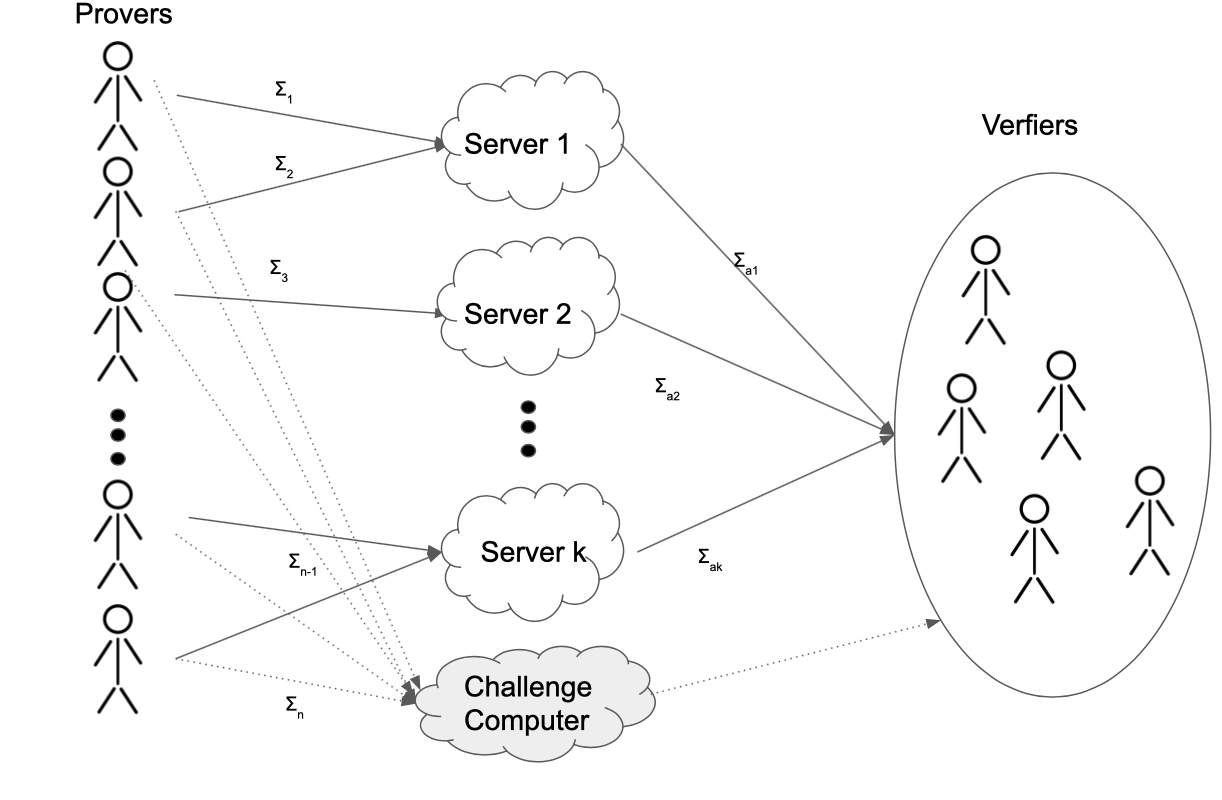
\includegraphics[width=\linewidth]{./figure/workflow_challanger.png}
\end{figure} 

\section{Completeness, Soundness and Zero-Knowledge}
%TODO intro
\subsection*{Trusted aggregating party}
This section will investigate if the proposed aggregated set membership proof presented in Construction \ref{alg:ZKSM-Agg}  fulfils the completeness, soundness and zero-knowledge requirements stated in Definition \ref{def:ZKP_agg} under the  assumption that the aggregation has been done according to equation \eqref{eq:aggDn} by one trusted party. 

Completeness follows from the argument given above, where it has been seen that $D\overset{?}{=}C^ch^{z_R}g^{z_x}$ given all parties where honest, and the completeness of the public signature based set membership proof. Thereby Construction \ref{alg:ZKSM-Agg} satisfies the completeness in Definition \ref{def:ZKP_agg}. 

Zero-knowledge follows directly from the zero knowledge property of Construction \ref{alg:ZKSM} and by realising that multiplying and adding elements which perfectly hides the secret $x_i$, with other elements independent of the secret will not reveal any information about the secret. This leads to that it remains to see if the soundness property holds for Construction \ref{alg:ZKSM-Agg}. 

The verification in Construction \ref{alg:ZKSM} consists of two equality checks. The first equality check $D\overset{?}{=}C^ch^{z_R}g^{z_x}$ convinces the verifier that the commitment and the proof element $z_x$ hides the same secret. The second equality check $a\overset{?}{=} e(V,y)^c(V,g)^{z_x}e(g,g)^{z_\tau}$ convinces the verifier that the secret used to compute $z_x$ is the same as the secret hidden in $V$ and the security of Bohen-Boyen signatures gives that this secret is a member of the set $\Phi$.  

Considering the second equality check of the set membership proof, that has not been aggregated, the soundness follows directly from the soundness of construction \ref{alg:ZKSM}. This is since this part of the proof is send directly from the provers to the verifier. 
%For the soundness of Construction \ref{alg:ZKSM-Agg} to hold, the verification of the aggregated proof $\Sigma_a$ should provide the same conviction to the verifier that all individual set membership proofs $\{\Sigma_i\}_{i\in\mathcal{S}}$. 

The equality check $D\overset{?}{=}C^ch^{z_R}g^{z_x}$ in the original set membership construction as seen above servers the purpose of ensuring the verifier that the secret hidden in the commitment $C$ is the same as the secret used to construct the value $z_x$. 
This property need to be checked that it remains after the aggregation. Meaning that the verifier should be sure that all secrets hidden in the commitments, are equal to the secrets used to compute the values $z_{x_i}$, in turn used in the aggregation to construct $z_x$. 
%TODO fix margin? ¨

To investigate this, consider two set membership proofs, $\Sigma_1$ and $\Sigma_2$, on the form $(V_i,a_i,D_i,z_{x_i},z_{\tau_i},z_{R_i) $ for $i=1,2$. Given these proofs and the Pedersen commitment published by the provers the trusted aggregating party computes $\Sigma_a= (\{V_1,V_2\},\{a_1,a_2\}, D,z_x,\{z_{x_1,}z_{x_2}\}, \{z_{\tau_1},z_{\tau_2}\}, z_R))$, according to algorithm \textbf{Aggregate} in construction \ref{alg:ZKSM-Agg}. Given this set up, it will be investigated if it can hold that: $D = (C_1C_2)^ch^{z_R}g^{z_x}}$, where $C_i = g^{\tilde{x}_i}h^{\tilde{R}_i}$ and $z_{x_i} = s_i-c_ix_i$ such that $x_i\neq \tilde{x}_i$ for $i$ equal to either $1$, $2$ or both. Resulting in that the below equations must be equal while assuming that $\tilde{x}_i\neq x_i$, 
\begin{align*}
LHS =& g^{s_1c_2+s_2c_1}h^{m_1c_2+m_2c_1}\\
RHS =& g^{c_1c_2(\tilde{x}_1+\tilde{x}_2)}h^{c_1c_2(\tilde{R}_1+\tilde{R}_2)} g^{ c_2(s_1-c_1x_1 ) + c_1(s_2-c_2x_2 ) } h^{ c_2(m_1-c_1R_1 ) + c_1(m_2-c_2\R_2 ) }\\
=&  g^{ s_1c_2+ s_2c_1} h^{ m_1c_2+ m_2c_1 }g^{c_1c_1 (\tilde{x}_1+ \tilde{x}_2) - c_1c_2 (x_1+x_2) } h^{ c_1c_1 (\tilde{R}_1+ \tilde{R}_2)-c_1c_2 (R_1+R_2) }.
\end{align*}
Under the assumption that the aggregation was done correctly, one of the following cases has to hold in order for $LHS=RHS$,
\begin{enumerate}
\item $x_1= \tilde{x}_2$ and $x_2 = \tilde{x}_1$
\item $(x_1+x_2) = (\tilde{x}_1+\tilde{x}_2)\: \text{mod} \: \Phi(N)$
\end{enumerate}

In the first case the provers are cheating, since they do not use the same secret in the commitments as in $z_{x_i}$. 
%If this is considered in the context of using the aggregated set membership proof in combination to a VAHSS construction the sum $y$ calculated in the VAHSS construction evaluates to the same value in both case $1$ and $2$, and all used terms in the summation is proved to be in the set $\Phi$. 
Despite cheating provers the result from the protocol is unaffected. This is since a cheating parties in this case only achieves to having their secret being committed to by another prover, as oneself commits to this prover's secret. It is not of relevance who committed what as long as all secrets is verified to be in the set. 

The second case shows that two provers can collaborate in such a way that they ensured the verifier that the secrets $x_1$ and $x_2$ are in the set, by falsely proven that the secrets in $x_1,x_2$ are equal to $\tilde{x}_i,\tilde{x}_2$. I.e the equality $D\overset{?}{=} ( \prod_{i=1}^2 C_i)^ch^{z_R}g^{z_x}$ holds true without $\tilde{x}_i=x_i$. Thereby using $\tilde{x}_1$ and $\tilde{x}_2$ belong to the set $\Phi$ and $x_1,x_2$ not being in the set, the provers has successfully cheated.
Thus it has to be assumed that provers cannot communicate in order for the soundness property to hold for the aggregated set membership. 

The arguments above for the soundness of Construction \ref{alg:ZKSM-Agg} is formally stated and proved in Theorem \ref{thm:CSV_aggreated}. 

\hspace{10pt}
\begin{thm}
\label{thm:CSV_aggreated}
Assumed that  the aggregation is done according to algorithm \textbf{Aggregate} in Constrcution \ref{alg:ZKSM-Agg} by a trusted party,  that provers cannot communicate and that the set membership proof in Construction \ref{alg:ZKSM} is sound according to Definition \ref{def:ZKP}. Then the aggregated set membership proof in Construction \ref{alg:ZKSM-Agg} satisfies the soundness in Definition \ref{def:ZKP_agg}. 
\end{thm}

\begin{proof}
 Let $T$ denote the index-set of malicious provers.  Assume that a prover $c_i$, $i\in T$ can construct a set membership proof for the Pedersen commitment $C_i = g^{\tilde{x}_i}h^{\tilde{R}_i}$ such that $\tilde{x}_i \neq x_i}$ and $z_{x_i}=s_i-c_ix_i$.

%TODO fixa mening
The soundness of set membership proofs implies that the values of the malicious provers proofs used in the non aggregated equality check has to be computed according to the algorithm \textbf{Prove} in Construction $\ref{alg:ZKSM-Agg}$.
%Thereby a malicious client has to commit values of $D_i,z_{R_i}$ such that after aggregation the the algorithm \textbf{VerifyAggregted} validates true while the Pedersen commitment $C_i$ and value $z_{x_i}$ are such that $x_i\neq\tilde{x_i}$, such that $x_i\in\Phi$ and $\tilde{x}_i \notin\Phi$.
Assume further that all honest provers computes their set membership proof according to \textbf{Prove} and for the malicious provers the set membership proof and Pedersen commitment must, due to the soundness of Construction \ref{alg:ZKSM}, fulfil:
\begin{align*}
V_i &= A_{x_i}^{\tau_i}\\
a_i &= e(V_i,g)^{-s_i}e(g,g)^{t_i}\\
D_i &= g^{\tilde{s}_i}h^{\tilde{m}_i}\\
z_{x_i} &= s_i-x_ic_i\\
z_{\tau_i} &= t_i- \tau_i c_i\\
z_{R_i} &\in\mathds{F}\\
C_i &= g^{\tilde{x}_i}h^{\tilde{R}_i},
\end{align*}
where $\tilde{x}_i\neq x_i$ and $x_i\in\Phi$. It is not required that $\tilde{s}_i =s_i$, $\tilde{m}_i =m_i$, $\tilde{R}_i =R_i$ nor required that they are not equal. 

In order for the algorithm \textbf{VerifyAggregated} to validate true it has to hold that $D=C^ch^{z_R}g^{z_x}$, where $D,z_R,z_x$ is the aggregation according to equation \eqref{eq:aggDn} of all provers, honest and malicious,  set membership proofs. For this to be an equality it has to hold that the left hand side and right hand side below are equal, 
\begin{comment}
\begin{equation}
\label{eq:}
\begin{aligned}
C &= \prod_{i\in T }  C_i  \prod_{i\in\mathcal{S}\backslash T }  C_i  =  \prod_{i\in T }  g^{\tilde{x}_i}h^{\tilde{R}_i}  \prod_{i\in\mathcal{S}\backslash T }  g^{x_i}h^{R_i} =  \prod_{i\in T }  g^{\tilde{x}_i}  \prod_{i\in\mathcal{S}\backslash T }  g^{x_i} 
 \\
D &=\prod_{i\in T }  D_i ^{\prod_{\substack{j\in\mathcal{S}\\ j\neq i}} c_j } \prod_{i\in\mathcal{S}\backslash T }  D_i ^{\prod_{\substack{j\in\mathcal{S}\\ j\neq i}} c_j }  =  \prod_{i\in T }  (g^{\tilde{s}_i}h^{\tilde{m}_i}) ^{\prod_{\substack{j\in\mathcal{S}\\ j\neq i}}  c_j } \prod_{i\in\mathcal{S}\backslash T }  (g^{s_i}h^{m_i}) ^{\prod_{\substack{j\in\mathcal{S}\\ j\neq i}}  c_j }
 \\
z_R &= \sum_{i\in T } \Big( \prod_{\substack{j\in\mathcal{S}\\ j\neq i}} c_j \Big) z_{R_i} +  \sum_{i\in\mathcal{S}\backslash T } \Big( \prod_{\substack{j\in\mathcal{S}\\ j\neq i}} c_j \Big) z_{R_i} \\
\end{aligned}
\end{equation}
\end{comment}

\begin{align*}
LHS =& D = g ^ {\sum_{i\in T } \Big(\prod_{\substack{j\in\mathcal{S}\\ j\neq i}}   c_j \Big)\tilde{s}_i + \sum_{i\in\mathcal{S}\backslash T } \Big(\prod_{\substack{j\in\mathcal{S}\\ j\neq i}}   c_j \Big)s_i} h^ {\sum_{i\in T } \Big(\prod_{\substack{j\in\mathcal{S}\\ j\neq i}}    c_j \Big)\tilde{m}_i+ \sum_{i\in\mathcal{S}\backslash T} \Big(\prod_{\substack{j\in\mathcal{S}\\ j\neq i}}    c_j \Big)m_i} 
 \\
RHS =& C^ch^{z_R}g^{z_x} =   \Big( g^{\sum_{i\in T} \tilde{x}_i + \sum_{i\in \mathcal{S}\backslash T} x_i} h^{\sum_{i\in T} \tilde{R}_i + \sum_{i\in \mathcal{S}\backslash T} R_i}  \Big) ^{\prod_{j\in\mathcal{S}} c_j}  h^{ \sum_{i\in T } \Big( \prod_{\substack{j\in\mathcal{S}\\ j\neq i}} c_j \Big) z_{R_i}}
 \\
& h^{\sum_{i\in\mathcal{S}\backslash T } \Big( \prod_{\substack{j\in\mathcal{S}\\ j\neq i}}   c_j \Big)m_i- \sum_{i\in\marhcal{S}\backslash T} \big( \sum_{i\in\mathcal{S}} c_j\big)R_i}  
g^{ \sum_{i\in\mathcal{S}} \Big( \prod_{\substack{j\in\mathcal{S}\\ j\neq i}}   c_j \Big)s_i - \big( \prod_{j\in\mathcal{S}} c_j \Big) \sum_{i\in\mathcal{S}} x_i}
\\ 
 =&  g ^{\prod_{j\in\mathcal{S}} c_j \big(\sum_{i\in T} \tilde{x}_i + \sum_{i\in T} x_i\big) +  \sum_{i\in T} \big( \prod_{\substack{j\in\mathcal{S}\\ j\neq i}} c_j\big) s_i     } h^{ \big( \prod_{j\in\mathcal{S}} c_j\big)\sum_{i\in T} \tilde{R}_i  + \sum_{i\in T } \Big( \prod_{\substack{j\in\mathcal{S}\\ j\neq i}} c_j \Big) z_{R_i}}
 \\
 & g ^ {\sum_{i\in\mathcal{S}\backslash T } \Big(\prod_{\substack{j\in\mathcal{S}\\ j\neq i}}   c_j \Big)s_i} h^ { \sum_{i\in\mathcal{S}\backslash T} \Big(\prod_{\substack{j\in\mathcal{S}\\ j\neq i}}    c_j \Big)m_i} 
\end{align*}
Both sides of the equality above can be interpreted as a Pedersen commitments.  It is assumed, under the discrete logarithm assumption, that two Pedersen commitments cannot be equal unless their arguments are equal. This implies that for the LHS to be equal to the RHS above the exponents of $g$ and $h$ has to be equal on both sides. Consider the exponent of $g$ this leads to,
\begin{align}
\label{eq:cheatingCient}
\sum_{i\in T} \big(\prod_{\substack{j\in\mathcal{S}\\ j\neq i}} c_j \big) \tilde{s}_j =& \prod_{j\in\mathcal{S}} c_j \big(\sum_{i\in T} \tilde{x}_i + \sum_{i\in T} x_i\big) + \sum_{i\in T} \big( \prod_{\substack{j\in\mathcal{S}\\ j\neq i}} c_j\big) s_i  . 
\end{align}

It remain to argue that equality in equation \eqref{eq:cheatingCient} cannot hold unless $\tilde{x}_i= x_i$, which would lead to an contradiction. 

First consider the case that the set $T$ only consist of one element, implying that there is only one malicious client. Without loss of generality assume that this is client $c_k$. Under this assumption equation \eqref{eq:cheatingCient} can be rewritten to, 
\begin{align*}
\big(\prod_{\substack{j\in\mathcal{S}\\ j\neq k}} c_j \big)  \tilde{s}_k  =& \big ( \prod_{\substack{j\in\mathcal{S}\\ j\neq k}} c_j \big)c_k \big( \tilde{x}_k + x_k\big) +\big( \prod_{\substack{j\in\mathcal{S}\\ j\neq k}} c_j\big) s_k  \implies   \tilde{s}_k  = c_k \big( \tilde{x}_k + x_k\big) + s_k
\end{align*}
If it would be possible to choose $\tilde{s}_k = c_k \big( \tilde{x}_k + x_k\big) + s_k $, it would be possible to cheat in the set membership in Construction \ref{alg:ZKSM}. Thereby if $|T|=1$, it must hold that $\tilde{x}_k=x_k$

%TODO define random more clear
Instead assume that $|T|>1$ and that $c_k$ is a malicious client. Under the assumption that the provers cannot communicate and collaborate other clients set membership proof, $\{\Sigma_i\}_{\substack{i\in\mathcal{S}\\ i\neq k}}$, can be seen as random values for prover $c_k$ during the construction of $\Sigma_k$. Therefore under this assumptions equation \eqref{eq:cheatingCient} can be rewritten to, 
\begin{align*}
\big(\prod_{\substack{j\in\mathcal{S}\\ j\neq i}} c_j \big) \tilde{s}_k +  \overbrace{\sum_{\substack{i\in T \\ i\neq k}} \big(\prod_{\substack{j\in\mathcal{S}\\ j\neq i}} c_j \big) \tilde{s}_j}^{\text{Random }}  &=
  \big ( \prod_{\substack{j\in\mathcal{S}\\ j\neq k}} c_j \big)c_k \big( \tilde{x}_k + x_k\big) +\big( \prod_{\substack{j\in\mathcal{S}\\ j\neq k}} c_j\big) s_k 
  \\ 
   &+ \overbrace{\prod_{j\in\mathcal{S}} c_j \big(\sum_{\substack{i\in T \\ i\neq k}} \tilde{x}_i + \sum_{\substack{i\in T \\ i\neq k}} x_i\big)}^{\text{Random}} \\
   & + \overbrace{\sum_{\substack{i\in T \\ i\neq k}} \big( \prod_{\substack{j\in\mathcal{S}\\ j\neq i}} c_j\big) s_i  }^{\text{Random}}
\end{align*}
If $\tilde{x}_k \neq x_k$, this would imply that the set membership proof can be broken by adding random values to $D$ and $z_x$ in Construction \ref{alg:ZKSM}. This is a contradiction to the soundness of set membership proofs. This implies that $\tilde{x}_k=x_k$. 

It has been proved that the aggregated set membership proof, presented in Construction \ref{alg:ZKSM-Agg}, fulfils the soundness in Definition \ref{def:ZKP_agg} under the assumptions that the aggregation is performed according to equation \eqref{eq:aggDn} by a trusted party, that provers cannot communicate and that the set membership proof in Construction \ref{alg:ZKSM} is sound. 
\begin{comment}
\begin{align*}
 \sum_{i\in T} \big( \prod_{\substack{j\in\mathcal{S} \\ j\neq i}} c_j \big) \tilde{m}_j =&  \prod_{j\in\mathcal{S}} c_j \big( \sum_{i\in T} \tilde{R}_i  \big)   + \sum_{i\in T} \big( \prod_{\substack{j\in\mathcal{S} \\ j\neq i}} c_j\big) z_{R_i}\\
  \big( \prod_{\substack{j\in\mathcal{S} \\ j\neq i}} c_j \big) \tilde{m}_k =& \big( \prod_{\substack{j\in\mathcal{S}\\ j\neq k}} c_j\big) c_k \big( \tilde{R}_k  \big)  + \big( \prod_{\substack{j\in\mathcal{S}  \\ j\neq k}} c_j\big) z_{R_k} \implies   \tilde{m}_k = c_k\tilde{R}_k  +  z_{R_k} .
  \\
  \big( \prod_{\substack{j\in\mathcal{S} \\ j\neq i}} c_j \big) \tilde{m}_k + \sum_{i\in T \\ i\neq k}} \big( \prod_{\substack{j\in\mathcal{S} \\ j\neq i}} c_j \big) \tilde{m}_j =&  \prod_{j\in\mathcal{S}} c_j \big( \sum_{i\in T} \tilde{R}_i  \big)   + \sum_{i\in T} \big( \prod_{\substack{j\in\mathcal{S} \\ j\neq i}} c_j\big) z_{R_i}
  \\
  & \Big( g^{c \sum_{i\in T} \tilde{x}_i } \Big)    h^{ \sum_{i\in T } \Big( \prod_{\substack{j\in\mathcal{S}\\ j\neq i}} c_j \Big) z_{R_i} } 
 h^{\sum_{i\in\mathcal{S}\backslash T } \Big( \prod_{\substack{j\in\mathcal{S}\\ j\neq i}}   c_j \Big)m_i- \sum_{i\in\marhcal{S}\backslash T} \big( \sum_{i\in\mathcal{S}} c_j\big)R_i}
   \\
& g^{ \sum_{i\in\mathcal{S}} \Big( \prod_{\substack{j\in\mathcal{S}\\ j\neq i}}   c_j \Big)s_i - c  \sum_{i\in T } x_i}
\end{align*}
\end{comment}
\end{proof}
% c be partially aggregated by servers, not compleatly by aggregator of RP -> alll c_i used most be correct?

%More precisely it has to hold that a secret not in $\Phi$ satisfies the verification with a negligible property and additionally that the secret hidden in the commitments $C_i$ is the same as the secrets in $z_{x_i}$. 


%Neither the  second equality test including  bilinear mapping holds after aggregation, this equality will not hold even if the challenges are equal, i.e $c_1=c_2$ unlike the first.  This concludes that the neither set membership nor signature based range proof can be straight forward aggregated without modifications.  Challange in included on both sides, is this an issue? But not yout own challange on LHS?

\subsection*{Untrusted Aggregating party }
In the previous section it was assumed that the algorithm \textbf{Aggregate} was performed correctly by a trusted party. Under the assumption that the proving parties cannot communicate is was argued that the aggregated set membership proof in Construction \ref{alg:ZKSM-Agg} satisfies the correctness, soundness and zero-knowledge property  in Definition \ref{def:ZKP_agg}.

In this section it will be investigated if the trusted party assumption is necessary or if some weaker assumption is sufficient alternatively if the aggregation can be checked. It will be assumed that proving parties cannot communicate between themselves and that proving parties cannot communicate with the aggregating party. 

Note that since all input to the algorithm \textbf{Aggregate} is public, the aggregation can be done by anybody. Therefore an aggregation performed can always be checked if it is correct by running the algorithm \textbf{Aggregate} on one's own and then examine if the results are the same. To aggregate the set membership proofs is an expensive operations and hence arguments on an aggregations correctness without having to redo the aggregation would be useful.

%An important feature in the verification of the original set membership construction is that verifier can compute the challenge as the hash of parts of the proof and hence the prover cannot cheat and use some cleaver challenge that cancel terms or in some other way affects the proof. The proposed aggregation does not provide sufficient input to the verification algorithm for the verifier to compute the individual challenges and then their product used in the verification. Further the challenges are computed and used in the aggregation hence it is necessary to perform some assurance that it is the correct challenges used. 

%TODO fix below
Before looking into how the aggregation party might cheat and depart from the aggregation in equation \eqref{eq:aggDn}, it will be cleared out what values the aggregation party can affect and what requirements that has hold. The aggregation party need to provide values for the proof parameters $D,z_x,z_R$ such that $D=C^ch^{z_R}g^{z_x}$. The party performing the aggregation can not modify the values of the product of commitments, denoted $C$, nor the value of the product of the provers challenges, denoted $c$.  If the aggregation can be performed  such that the  values $D,z_x,z_R$ are not computed according to equation \eqref{eq:aggDn} and the verification verifies true, the aggregating party has deceived the verifier.

An important distinction is that in the original set membership construction the value of the challenge, $c_i$, used is not know when constructing $C_i,V_i,D_i,a_i$ since it is a function of these values. In the aggregated set membership the challenges depends on the values publicly known for the aggregating party. This leads to that this knowledge can be taken advantage of to cheat. This results in that besides having a party independent of the aggregation, possibly the verifier, computing the product of the challenges, it must also be verified that $D\neq C^c$, where $C=\prod_{i\in\mathcal{S}}C_i$ and $c=\prod_{i\in\mathcal{S}}c_i$.

If it is not checked that $D \neq C^c$ it would be possible to choose the values $D,z_x,z_R$ according to,
\begin{align*}
D =& \prod_{i\in\mathcal{S}} C_i ^{\prod_{i\in\mathcal{S}} c_i}	\\
z_x =& \phi(p)	\\
z_R =& \phi(p),	\\
\end{align*}
where $p$ is the prime underlying the field $\mathds{F}$. For the above choice of $D,z_x,z_R$ the equation, $D\overset{?}{=} \big(\prod_{i\in\mathcal{S}}^nC_i\big)^{\prod_{i\in\mathcal{S}}^n c_i} h^{z_R}g^{z_x}$ holds trivially true, independent of whether the commitment $C_i$ and the values $z_{x_i}$ hides the same secret for all $i\in\mathcal{S}$. Henceforth it will be assume that it is checked that $D \neq C^c$.


This leads to that the aggregated values $D,z_R,z_x$  must be such that $D \neq C^c$ and that left hand side equals the right hand side in the below equation system:

\begin{align*}
LHS =& D\\
RHS  =& \big(\prod_{i\in\mathcal{S}}C_i\big)^{\prod_{i\in\mathcal{S}} c_i} h^{z_R}g^{z_x} =
\big( g^{\sum_{i\in\mathcal{S}} x_i } h^{\sum_{i\in\mathcal{S}} R_i} \big) ^{\prod_{i\in\mathcal{S}} c_i}h^{z_R} g^{z_x} \\
=& \big( g^{ (  \prod_{i\in\mathcal{S}} c_i ) \sum_{i\in\mathcal{S}} x_i ) } h^{ ( \prod_{i\in\mathcal{S}}  c_i ) \sum_{i\in\mathcal{S}} R_i ) } \big)h^{z_R} g^{z_x}.
\end{align*}

%In the original set membership construction is that the verifier uses the same value $z_x$ is used for the entire verification. In the aggregated set membership, an aggregated value $z_x$ is used to test if $D\overset{?}{=}C^ch^{z_R}g^{z_x}$ while non-aggregated values $z_{x_i}$ are used to verify $a_i=e(V_i,y)^ce(V_i,g)^{-z_x}e(g,g)^{z_{\tau_i}}$ for $i\in\mathcal{S}$. Thereby the same value is not used in the entire verification. This means that in the aggregated set membership the aggregated value $z_x$ has less claims that needs to be fulfilled in order for the verification to succeed. 

In order to have equality between the left hand side and the right hand side, the terms derived from the commitments must be cancelled. The aggregating party does not know the secrets $x_i$ or the random values $R_i$ for any $i\in\mathcal{S}$ nor the sums $\sum_{i\in\mathcal{S}} x_i$ and $\sum_{i\in\mathcal{S}} R_i$, this follows from the assumption that the provers cannot communicate with each-other or with the party performing the aggregation. 

Under the assumption discussed above, Theorem \ref{thm:aggrgeation} states that aggregation must be performed according to the algorithm \textbf{Aggregate} for the algorithm \textbf{Verify} to verify true in Construction \ref{alg:ZKSM-Agg}. 


% The argument is that in order to cancel the terms depending on the unknown sum of secrets, $x_i$, and random values, $R_i$, the values $z_{x_i}$ and $z_{R_i}$ must be used. These term can not be combined in a way that all cross terms are cancelled besides as in equation \ref{eq:aggDn}. Remark here that this is assumed and not proved, in other words the security of the aggregated set membership presented in Construction \ref{alg:ZKSM-Agg} is based on this assumption or alternatively as in the previous section the assumption that the aggregation is done by a trusted party.

\hspace{10pt}
\begin{thm}[\textbf{Security of aggregation without trusted third party assumption}]
\label{thm:aggrgeation}

Let $\mathcal{A}$ be a PPT adversary. Assume $\mathcal{A}$ knows 
the set membership proofs $\Sigma_i$ for $i\in\mathcal{S}$, where $\Sigma_i=(V_i,a_i,D_i,z_{x_i},z_{\tau_i},z_{R_i})$ calculated according to the algorithm \textbf{Prove} in Construction \ref{alg:ZKSM-Agg}. In addition the adversary has also knowledge of the Pedersen commitments $C_i$ and the challenges $c_i=Hash(D_i,a_i)$ for all $i\in\mathcal{S}$.\\
\\
Assume that the adversary  $\mathcal{A}$ cannot communicate with the provers and that the provers cannot communicate with each other,. This leads to that the  $\mathcal{A}$ has no knowledge of the secrets $x_i$ or the randomness $R_i$ in the Pedersen commitment, nor the sum of the secrets and random values. \\
\\
Under these assumptions the adversary $\mathcal{A}$ has a negligible probability of choosing $D,z_x,z_R$ such that: $D = C^cg^{z_x}h^{z_R}$, where $D\neq C^c$, $C=\prod_{i\in\mathcal{S}}C_i$ and $c=\prod_{i\in\mathcal{S}}c_i$ and  $z_x \neq \sum_{i\in\mathcal{S}} \Big( \prod_{j\in\mathcal{S}, j\neq i} c_j \big) z_{x_i}$. 

%The aggregated set membership proof, given in Construction \ref{alg:ZKSM-Agg}, fulfils the soundness in Definition \ref{def:ZKP} if the probability that the adversary $\mathcal{A}$ can cheat, according to the above definition, is negligible. 

%The adversary has successfully cheated if the values $D,z_x,z_R$ can be chosen such that $z_{x} \neq \sum_{i\in\mathcal{S}} \Big( \prod_{j\in\mathcal{S}, j\neq i} c_j \big) z_{x_i}$, or if they can be chosen in any other way then according to equation \eqref{eq:aggDn}. 

%The following is the informal description of the security proof\\
%\textbf{Known to the adversary:}\\
%The adversary has knowledge of the set membership proofs $RP_i$ for $i\in\mathcal{S}$, where $RP_i=(V_i,a_i,D_i,z_{x_i},z_{\tau_i},z_{R_i})$ calculated according to the algorithm \textbf{Prove} in Construction \ref{alg:ZKSM-Agg}. The adversary has also knowledge of the Pedersen commitments $C_i$ published by the provers and can calculate the challenges $c_i=Hash(D_i,a_i)$ for all $i\in\mathcal{S}$.\\
%\textbf{Not known:}\\
%The sums $\sum_{i\in\mathcal{S}} x_i$ and $\sum_{i\in\mathcal{S}}R_i$ are unknown just as the individual values $x_i$ and $R_i$ for all $i\in\mathcal{S}$, these are the values in the commitments $C_i=g^{x_i}h^{R_i}$.  The adversary cannot communicate with the provers. \\
%\textbf{Goal:}\\
%Given this information, the adversary wish to choose the values $D,z_x,z_R$ such that the equality $D = C^cg^{z_x}h^{z_R}$ holds and $D\neq C^c$, where $C=\prod_{i\in\mathcal{S}}C_i$ and $c=\prod_{i\in\mathcal{S}}c_i$.
%The adversary has successfully cheated if the values $D,z_x,z_R$ can be chosen such that $z_{x} \neq \sum_{i\in\mathcal{S}} \Big( \prod_{j\in\mathcal{S}, j\neq i} c_j \big) z_{x_i}$, or if they can be chosen in any other way then according to equation \eqref{eq:aggDn}. 
\end{thm}
\begin{proof}
Assume that the values $D,z_x,z_R$ may be chosen by the adversary, such that $D\in\mathds{G}$, $z_x,z_R\in\mathds{F}$ and  $z_x \neq \sum_{i\in\mathcal{S}} \Big( \prod_{j\in\mathcal{S}, j\neq i} c_j \big) z_{x_i}$. Assumes without loss of generality that  $D=g^ah^b$, where $a,b\in\mathds{F}$. Given this the adversary $\mathcal{A}$ needs to choose the values $a,b,z_x,z_R$ such that:
\begin{align*}
g^a h^b  = C^cg^{z_x}h^{z_R},
\end{align*}
% \Big(=  \big(g^{\sum_{i\in\marhcal{S}}x_i}h^{\sum_{i\in\mathcal{S}} R_i} \big)^c g^{z_x}h^{z_R} \Big) = 
the values of $C^c= \big(g^{\sum_{i\in\marhcal{S}}x_i}h^{\sum_{i\in\mathcal{S}} R_i} \big)^{\prod_{j\in\mathcal{S}}c_j} $ can not be modified by the adversary since they are send directly from the provers to the verifier and used in the verification.

Expanding the right hand side of the equality it follows that,
\begin{align*}
g^ah^b =  g^{c \sum_{i\in\mathcal{S}}x_i +z_x } h^{ c \sum_{i\in\mathcal{S}}R_i +z_R   }.
\end{align*}

If $a\neq c\sum_{i\in\mathcal{S}}x_i+z_x$ and $b\neq c\sum_{i\in\mathcal{S}}R_i +z_R$, the above is contradiction to the assumption that it is not possible to construct two equal Pedersen Commitments hiding different secrets. 

Thus the adversary must choose $a,b,z_x,z_R$ such that $a =  c\sum_{i\in\mathcal{S}}x_i+z_x$ and $b =  c\sum_{i\in\mathcal{S}}R_i +z_R$.  Considering the first equation it can be rewritten $a-z_x =  c \sum_{i\in\mathcal{S}} x_i \:\text{mod}\:\Phi(p)$ and then the second equation $b-z_R =  c \sum_{i\in\mathcal{S}} R_i \:\text{mod}\:\Phi(p)$. The right hand side of these equations is assumed to unknown, thereby the adversary has a negligible probability of choosing $a,b,z_x,z_R$ such that the above is satisfied. Thereby it follows that  $z_x = \sum_{i\in\mathcal{S}} \Big( \prod_{j\in\mathcal{S}, j\neq i} c_j \big) z_{x_i}$, which contradicts the assumption and proves the theorem. 


%This leads to that they must be chosen in a way such that the terms provided by $C^c$ is cancelled such that the two sides are equal, since it is assumed that $D\neq C^c$. This leads to that $z_x,z_R\neq 0$.

%Assumes w.l.o.g that $D=g^ah^b$, then if follows that $a,b,z_x,z_R$ must be chosen such that,
%\begin{align*}
%g^ah^b =  g^{c \sum_{i\in\mathcal{S}}x_i +z_x } h^{ c \sum_{i\in\mathcal{S}}R_i +z_R   }.
%\end{align*}
%If $a\neq c\sum_{i\in\mathcal{S}}x_i+z_x$ and $b\neq c\sum_{i\in\mathcal{S}}R_i +z_R$, the above is contradiction to the assumption that it is not possible to construct two equal Pedersen Commitments hiding different secrets. 

%Instead assume $a =  c\sum_{i\in\mathcal{S}}x_i+z_x$ and $b =  c\sum_{i\in\mathcal{S}}R_i +z_R$.  For the first equality to hold has to choose $a,z_x$ such that $a-z_x =  c \sum_{i\in\mathcal{S}} x_i \:\text{mod}\:\Phi(p)$. However the right hand side of this equation is assumed to unknown to the adversary and thus to have equality the adversary has aggregate according to equation \eqref{eq:aggDn}

%My idea is to argue that choosing the values in such a way would mean that the adversary has managed to construct two Pedersen commitments ($\mathds{E}(a,b)= g^ah^b$) such that $\mathds{E}(x,R)= \mathds{E}(x',R')$  but $x\neq x'$. 
\end{proof}

Note thate the Theorem would hold even if several untrusted parties would aggregate subsets if the proofs and then one verifier would verify all the aggregated proofs. 

%TODO read above and includeref to contsuction 8. 



%The arguments given for the assumptions of the aggregating party and arguments for the aggregated proof satisfying the completeness, soundness and zero knowledge  does not act as formal proofs, it should rather be seen an as motivations. therefore all potential attacks on aggregated set membership proof can not be deducted and before using it in practise further security checks need to be performed. 




%\subsection*{Aggregating Bulletproofs}
 %The original paper about Bulletproofs \cite{bulletProofs_theory} presents a method to aggregate Bulletproofs such that $n$ parties each having a Pedersen commitment $C_i,\: i=1,...,n$ can generate a single Bulletproof verifying that each commitment hides a secret in an allowed range. The presented approach only works if all parties uses the same challenge $c$ in the proof construction, this is achieved by introducing a dealer. During the constructions of the proofs when computing the challenges each client sends their proof of to this point to the dealer who aggregates the proofs and computes the challenges based on the aggregated proofs. For example, assume $n$ clients and denote their respective proofs with a subscript $i$, then to compute the challenges $y_i$ in construction \ref{alg:bullet} instead of each client computing $y_i = Hash(A_i,S_i)$, each client sends $A_i,S_i$ to the dealer who adds then homomorphically $A = \prod_{i=1}^n A_i, S = \prod_{i=1}^n S_i$ and the send back the challenge $y =Hash(A,S)$ to be use by all clients. This procedure is repeated for each challenge. 
 
 %It is noted that although the Fiat-Shamir heuristic is used to generate the challenges the construction is interactive since communication between the dealer and the clients is required during the construction of the aggregated range proof. If this procedure was ignored and each client instead computed their own challenges via Fiat-Shamir heuristic and the proof where aggregated after they were fully constructed,  then the challenges would differ between parties and the verification fail. 

%Concluding, it has been seen that the  Bulletproof can be aggregated with the cost on an  interactive construction, however this is not a desirable property for the the server and client verifiable AHSS. Investigation about whether this construction can be modified to be completely non-interactive has not been done and remains an open question.  

%This concludes that neither of the considered range proofs has be sucessfully fully aggregated aggregated  such that the verifier can perform one single verification instead of one for each client, at least not without some cost. Remark that this conclusion is not final and their may very well exist small or large modifications of the range proof that will allow them to be aggregated and still remaining non-interactive. The investigation of such modification is outside the scope of this paper but the reader is endorsed to explore this possibility. 
